\section{Zielsetzung}
In diesem Versuch wird der Effekt der Faraday Rotation verwendet um die
effektive Masse der Leitungselektronen in n-dotierten Galliumarsenid zu messen.

\section{Theorie}
In diesem Versuch scheint eine polarisierte elektromagnetische Welle durch
einen Halbleiter. Dieser Halbleiter wird einem Magnetfeld ausgesetzt was zu
einer Verdrehung der Polarisationsachse führt. Diese Begriffe werden im
folgenden definiert

\subsection{Halbleiter \cite[][Kap. 14]{book:expi3}}
Elektronen in Festkörpern haben anstelle von diskret definierten Zuständen
aufenthaltswahrscheinlichkeiten in der Form von Bändern. Leitende Festkörper
zeichnen sich durch Elektronen im ungebundenen Zustand aus. Isolatoren wiederum
haben eine große Bandlücke zwischen den Gebundenen Elektronen und dem ersten
freien Leitungsband. Diese Bandlücke ist bei Halbleitern in der Größenordnung
von etwa $\qty{1}{\eV}$. Die Bandstruktur von Halbleitern ist auch eine Funktion
des Impuls der Elektronen bzw. deren Wellenvektor $\vec{k}$

\subsection{Effektive Masse \cite[][Kap. 14]{book:expi3}}
Die Effektive Masse ist relevant für die Bewegungsgleichungen der Elektronen im
Leitungsband von Halbleitern sowie der Elektronen löcher im Valenzband. Sie
kann anstelle der Masse eines freien Elektrons verwendet werden. Sie ist
definiert als
\begin{align}
	m^* & = \hbar^2 \cdot \frac{d²E}{d k_i d k_j}
\end{align}

\subsection{Zirkulare Doppelbrechung \cite{man_a}}
\begin{figure}[H]
	\centering
	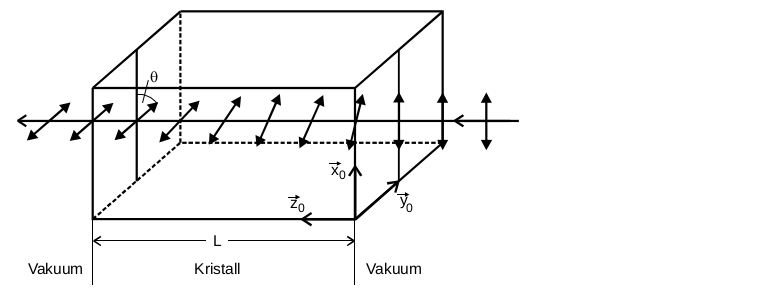
\includegraphics[width=0.8\textwidth]{./Bilder/zirpol.png}
	\caption{Zirkulare Polarisation \cite{man_a} }\label{fig:zirpol}
\end{figure}

Bestimmte Kristalle können die Polarisationsebene eines Linear polarisierten
Lichtstrahls drehen. dies kann dadurch erklärt werden, dass der Brechungsindex
für links und für rechtszirkular Polarisiertes licht unterschiedlich sind. Es
ist möglich das linear polarisierte Licht in eine rechts und eine linkszirkular
polarisierte Welle zu zerlegen.
\begin{align}
	E(z)    & = \frac{1}{2}(E_R(z) + E_L(z))                   \\
	E_R (z) & = (E_0 \vec{x}_0  - i E_0 \vec{y}_0) e^{i k_R z} \\
	E_L (z) & = (E_0 \vec{x}_0  + i E_0 \vec{y}_0) e^{i k_L z} 
\end{align}

Mit den Abkürzungen $ \psi := \frac{L}{2} (k_R + k_L)$ und
\begin{align}
	\theta & := \frac{L}{2} (k_R -k_L)                                    \\
	\intertext{ergibt sich für die Polatisationsebene am Ende des Kristalls mit der Länge $L$}
	E(L)   & = E_0 e^{i\psi} (\cos\theta \vec{x}_0 + sin\theta \vec{y}_0)
\end{align}
Die Phasengeschwindigkeit der Welle kann im allgemeinen durch die relation $V_{Ph}=\omega/k$
ausgedrückt werden. Es folgt
\begin{align}
	\theta &= \frac{L \omega}{2c} \left(\frac{1}{V_{Ph_R}} - \frac{1}{V_{Ph_L}}\right).
	\intertext{Das lässt sich auch bezogen auf die Brechungsindices mit 
	der Vakuumlichtgeschwindigkeit $c$ mit $n = c/v_{Ph}$ darstellen}
	\theta = \frac{L\omega}{2c}(n_R -n_L)
\end{align}

\subsection{Berechnung der Doppelbrechung in einem anisotropen Medium \cite{man_a} }
Die 


\subsection{Berechnung des Rotationswinkels der Polarisationsebene beim Faraday Effekt \cite{man_a} }
Die Bewegungsgleichung für ein gebundenes Elektron in einem Festkörper lautet
\begin{align}
	m \frac{d² \vec{r}}{d t²} + K \vec{r} = -e_0 \vec{E}(\vec{r}) \frac{d \vec{r}}{dt} \times \vec{B}.
\end{align}
$K$ ist hierbei eine Konstante.
Aus der Beschreibung dieser Gleichung im Sinne des Verschiebungsstroms $\vec{P} = -N e_0 \vec{r}$
mit N der Ladungsdichte
und einem Elektrischen Feld der Form $\vec{E} = e^{- i \omega t}$ ergibt sich für große $\omega$
\begin{align}
	-m\omega² \vec{P} + K \vec{P} = e_0^2 E_y -i e_0 \omega \vec{P} \times \vec{B}
\end{align}
Berechnungen mit dem Magnetisierungstensor $\chi$ in \cite{man_a} ergibt sich für den Winkel Theta
die Form
\begin{align} % Es fehlt hier noch die verbindung \chi zu brechungsindizes 
	\theta = \frac{e_0^3 \omega² NBL}{2 \epsilon_0 c(-m\omega²+ K)² -(e_0 \omega B)}
\end{align}

Vielleicht braucht man ja diese Formeln:
\begin{align}
	E                 & = E_L + \frac{\hbar k²}{2 m_e}                 \\
	\frac{d v_g}{d t} & = \frac{1}{\hbar^2}\frac{d^2 E}{d^2 k} \vec{F} \\
	E_e(\vec{k})      & = \frac{\hbar²}{3m^*_e}
\end{align}

\subsection{Fehlerrechnung}
Für die Fehlerrechnung werden alle \textbf{Mittelwerte} von $N$ Messungen
folgendermaßen berechnet:

\begin{equation}
	\overline{x} = \frac{1}{N} \cdot \sum_{i=1}^N x_i
	\label{eqn:Mittelwert}
\end{equation}

und alle \textbf{Standardabweichungen zum Mittelwert} mit:

\begin{equation}
	\increment\overline{x} = \sqrt{\frac{1}{N\cdot(N-1)}\cdot\sum_{i=1}^N (x_i-\overline{x})^2}
	\label{eqn:St_Mittelwert}
\end{equation}

Der Fehler für zusammenhängende Messwerte wird dann mit der \textbf{Gaußschen
	Fehlerfortpflanzung} berechnet:

\begin{equation}
	\increment{f} = \sqrt{ \sum_{i = 1}^{N}  \biggl(\frac{\partial{f}}{\partial{x_i}}\biggr)^2\cdot(\increment{x_i})^2}
	\label{eqn:Gauss}
\end{equation}

Die Fehlerfortpflanzung wird mit Uncertainties in Python \cite{uncertainties}
ermittelt.

%---------------------------------------------------------------------------------------------------------------------------------------------------------------%

\section{Durchführung\cite{man}}% TODO Zahlen überprüfen
Zwei Spulen werden hintereinander mit einem konstanten Strom von
$\qty{10}{\ampere}$ versorgt. Eine Hallsonde wird durch die Spule geschoben um
die Magnetfeldverteilung zu messen. Die Proben werden im Versuch in der
Mitte der Spule eingespannt wo das Magnetfeld am stärksten ist.

Der Versuch wird wie in Abbildung \ref{fig:aufbau} aufgebaut. Weißes licht wird
in einem einstellbaren Polarisator polarisiert und scheint durch die Spule. Im
Zentrum der Spule wird bei dem höchsten Magnetfeld eine Probe mit einer
bekannten Elektronenlochdichte eingespannt. Das Licht fällt danach auf ein
Glen-Thomson Prisma. Es spaltet das Licht in zwei Teile mit zueinander
senkrechter linearer Polarisation. Die beiden Photowiderstände geben ihr Signal
weiter an einen Differenzverstärker. Dessen Signalspannung ist proportional zu
dem Intensitätsunterschied zwischen den beiden Polarisationsachsen. Wenn die
Signalspannung des Differenzverstärkers null (bzw. minimal) wird, ist die
Polarisation genau diagonal zu dem Prisma. Um das Rauschen der Photowiderstände
von dem Lichtsignal zu unterscheiden wird zusätzlich der % Hier die Sorten der Proben einfügen

Der Faraday Effekt rotiert die Polarisationsebene des Lichtes um den Winkel
$\theta$. Das mit einem Goniometer einstellbare Glen-Thomson-Prisma wird auf
den Winkel gedreht, bei dem die Differenzspannung minimal ist.

\begin{figure}
	\centering
	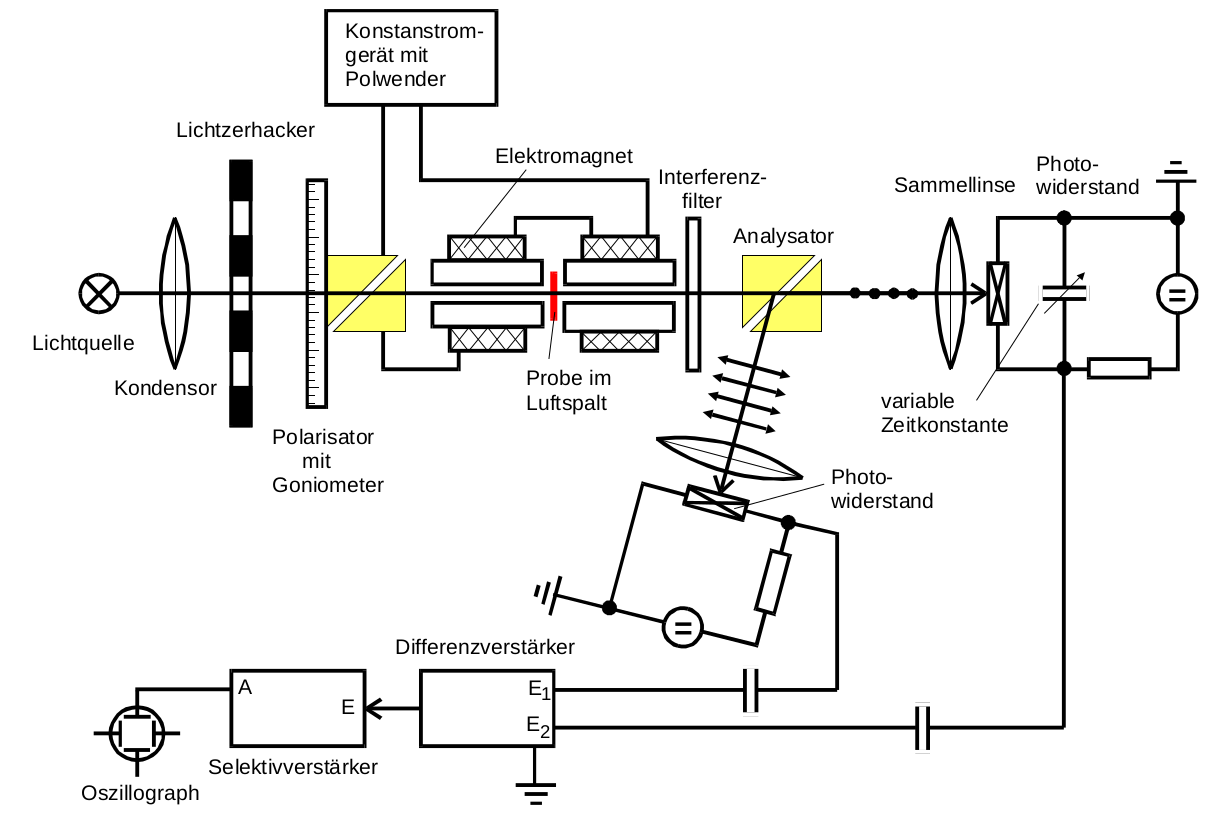
\includegraphics[width=0.8\textwidth]{./Bilder/aufbau.png}
	\caption{Der Versuchsaufbau \cite{man}}\label{fig:aufbau}
\end{figure}

